%
% Generated at 10.03.2023 - 16:20:16 by QConnectionWinapp
%

\emph{QConnectionWinapp}

\hypertarget{prerequisites}{%
\section{Prerequisites}\label{prerequisites}}
To use the QConnectWinapp library, users need to install the following app prerequisites:

WinAppDriver: https://github.com/Microsoft/WinAppDriver/releases (version \>\=1.2.1)

Windows SDK: https://developer.microsoft.com/en-us/windows/downloads/windows-sdk/

\hypertarget{getting-started}{%
\section{Getting Started}\label{getting-started}}

You can checkout all
\href{https://github.com/test-fullautomation/robotframework-qconnect-winapp/}{QConnectWinapp}
sourcecode from the GitHub.

After checking out the source completely, you can install by running
below command inside \textbf{robotframework-qconnect-winapp} directory.

\begin{verbatim}
python setup.py install
\end{verbatim}

\hypertarget{usage}{%
\section{Usage}\label{usage}}

QConnectWinapp is a backend extension for the QConnectBase library that adds support for testing WinApp UI.
From the user's perspective, this means they now have an additional connection type for WinApp testing when using the \textbf{connect} keyword in the QConnectBase library.
With QConnectWinapp, users can now easily automate tests for Windows desktop applications, and take advantage of its integration with WinAppDriver to interact with UI elements and validate their behavior.

Please refer to \href{https://github.com/test-fullautomation/robotframework-qconnect-base/blob/develop/QConnectBase/QConnectBase.pdf}{QConnectBase} for more information on how to use the \textbf{connect} keyword.
In this section, we will focus on the \textbf{Winapp} connection type and how to configure it.

\hypertarget{connect}{%
\subsection{\texorpdfstring{\textbf{Configurations for Winapp connection type}}{connect}}\label{connect}}

QConnectBaseLibrary has already
supported below connection types:

\begin{quote}
\begin{itemize}
\tightlist
\item
  \textbf{TCPIPClient}: Create a Raw TCPIP connection to TCP Server.
\item
  \textbf{SSHClient}: Create a client connection to a SSH server.
\item
  \textbf{SerialClient}: Create a client connection via Serial Port.
\item
  \textbf{DLT}: Create a client connection to Diagnostic Log and Trace(DLT) Module.
\end{itemize}
\end{quote}

QConnectWinapp add one more connection type for Winapp UI testing call \textbf{Winapp}


Below is the description of the configuration string for Winapp connection type:


\begin{robotcode}
{
    "host": [host ip],     # Optional. Default value is "localhost".
    "port": [listening port]  # Optional. Default value is 4723.
    "caps": [Desired Capabilities string in JSON format],  # E.g. { "app": "C:/Program Files/BOSCH/CMST/CMST.exe"}
    "logfile": [Log file path. Possible values: 'nonlog', 'console', [user define path]]
}
\end{robotcode}

\begin{table}[h]
\centering
\caption{List of Capabilities}
\begin{tabular}{|p{3cm}|p{9cm}|}
\hline
\textbf{Capability} & \textbf{Description} \\
\hline
app & The package full name or the executable file's full path of the application to automate (e.g. Microsoft.WindowsCalculator\_8wekyb3d8bbwe!App). \\
\hline
deviceName & Mostly optional, but the name of your device \\
\hline
automationName & The name of the automation engine to use (e.g. windows). \\
\hline
\end{tabular}
\end{table}

\hypertarget{definition}{%
\subsection{\texorpdfstring{\textbf{How to define a GUI control}}{definition}}\label{definition}}
Currently, the QConnectWinapp library supports identifying a GUI control on a test application through its Accessible Name. There are various ways to determine the accessible name of a control, one of which is by using the Inspect.exe tool. To use it, follow these steps:
\begin{itemize}
\item Navigate to the Windows SDK folder located under C:\textbackslash Program Files (x86)\textbackslash Windows Kits\textbackslash 10\textbackslash bin\textbackslash 10.0.17134.0\textbackslash x64
\item Open Inspect.exe
\item Hover over the control you want to identify on the test application
\item In the right-hand pane of Inspect.exe, you will be able to determine the Accessible Name of the control by its AutomationId property.
\end{itemize}

\begin{figure}[h]
  \centering
  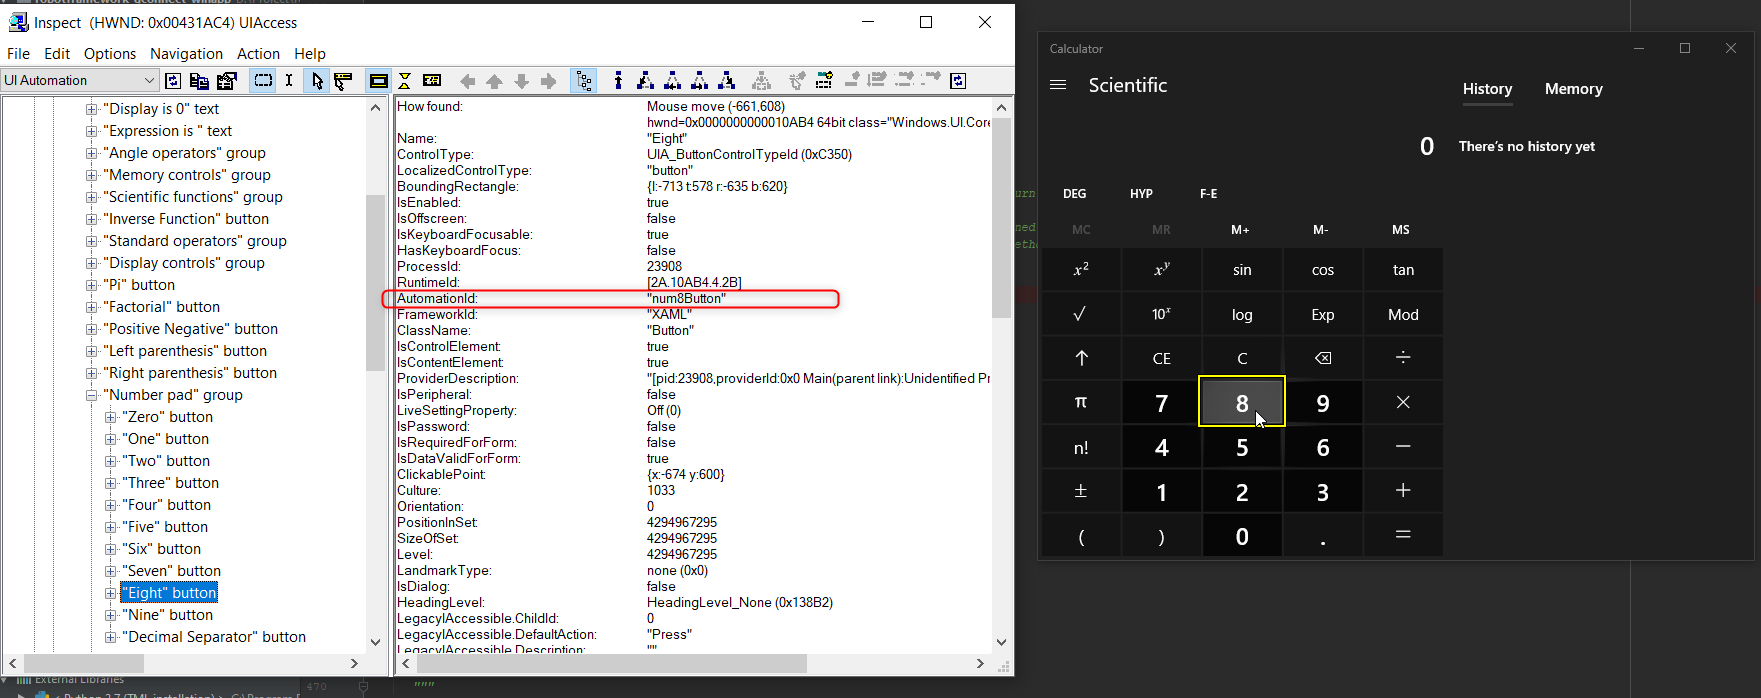
\includegraphics[width=\linewidth]{pictures/capture_control.png}
  \caption{Using Inspect.exe to identify the Accessible Name of Number 8 button.}
\end{figure}

\hypertarget{example}{%
\section{Example}\label{example}}
In this example, I provide a test scenario that allows adding on the Calculator app as follows: the script will open the Calculator application on Windows, then press the '8' button, press the '+' button, press the '9' button, and then press the '=' button.
Then, verify if the result textbox displays the result '17'.


\begin{robotcode}
*** Settings ***
Documentation    Suite description
Library     QConnectBase.ConnectionManager
Resource    QConnectWinapp/GUIAction.resource

*** Variables ***
${CONNECTION_NAME}  TEST_CONN

&{Number 8}       acc_id=num8Button
&{Number 9}       acc_id=num9Button
&{Equal}          acc_id=equalButton
&{Result}         acc_id=CalculatorResults
&{Plus}           acc_id=plusButton


*** Test Cases ***
Test Adding
    ${config_string}=    catenate
    ...  {\n
    ...         "host":   "localhost",\n
    ...         "port": 4723,\n
    ...         "caps":\n
    ...         {\n
    ...               "app": "Microsoft.WindowsCalculator_8wekyb3d8bbwe!App"\n
    ...         }\n
    ...  }\n

    log to console       \nConnecting with below configurations:\n${config_string}
    ${config}=             evaluate        json.loads('''${config_string}''')    json

    connect             conn_name=${CONNECTION_NAME}
    ...                 conn_type=Winapp
    ...                 conn_conf=${config}

    send command        conn_name=${CONNECTION_NAME}
    ...                 element_def=${Number 8}
    ...                 command=${Action.click}

    Sleep    1s

    send command        conn_name=${CONNECTION_NAME}
    ...                 element_def=${Plus}
    ...                 command=${Action.click}

    Sleep    1s

    send command        conn_name=${CONNECTION_NAME}
    ...                 element_def=${Number 9}
    ...                 command=${Action.click}

    Sleep    1s

    send command        conn_name=${CONNECTION_NAME}
    ...                 element_def=${Equal}
    ...                 command=${Action.click}

    ${res}=     verify     conn_name=${CONNECTION_NAME}
    ...                    element_def=${Result}
    ...                    search_pattern=17
    ...                    send_cmd=${Action.get_text}
    ...                    timeout=20

    log to console  \nCalculation result: ${res}[0]


*** Keyword ***
Close Connection
    disconnect  ${CONNECTION_NAME}
\end{robotcode}

\textbf{Explanation:}
\begin{itemize}
\item \colorbox{gray!16}{\textbf{\&\{Number 8\} acc\_id=num8Button}}: This line is used to identify the 'Number 8' button as the control on the application with an Accessible Name (acc\_id) of 'num8Button'.
\item \colorbox{gray!16}{\textbf{"app": "Microsoft.WindowsCalculator\_8wekyb3d8bbwe!App"}}: This line specifies that the AUT is the application with the package name 'Microsoft.WindowsCalculator\_8wekyb3d8bbwe!App'. You can also use the full path to the exe file of the AUT.
\item \colorbox{gray!16}{\textbf{send command conn\_name=\$\{CONNECTION\_NAME\}...command=\$\{Action.click\}}}: This line means to click on the Number 8 button on the AUT.
\item \colorbox{gray!16}{\textbf{\$\{Action.click\}}} has been defined in the resource file \colorbox{gray!16}{\textbf{QConnectWinapp/GUIAction.resource}}.

Currently supported in the GUIAction.resource:
\begin{table}[h]
    \centering
    \begin{tabular}{|l|l|}
        \hline
        \textbf{Action} & \textbf{Description} \\ \hline
        \$\{Action.click\} & Clicks on a GUI element \\ \hline
        \$\{Action.get\_text\} & Gets the text of a GUI element \\ \hline
        \$\{Action.get\_visible\} & Get the visibility of a GUI element \\ \hline
        \$\{Action.get\_enable\} & Check if a GUI element is eanbled \\ \hline
    \end{tabular}
    \caption{Actions supported in GUIAction.resource}
    \label{tab:actions}
\end{table}


\end{itemize}


\hypertarget{contribution-guidelines}{%
\section{Contribution Guidelines}\label{contribution-guidelines}}

QConnectBaseLibrary is designed for ease of making an extension library.
By that way you can take advantage of the QConnectBaseLibrary's
infrastructure for handling your own connection protocal. For creating
an extension library for QConnectBaseLibrary, please following below
steps.

\begin{enumerate}
\def\labelenumi{\arabic{enumi}.}
\tightlist
\item
  Create a library package which have the prefix name is
  \textbf{robotframework-qconnect-}\emph{{[}your specific name{]}}.
\item
  Your hadling connection class should be derived from
  \textbf{QConnectionLibrary.connection\_base.ConnectionBase} class.
\item
  In your \emph{Connection Class}, override below attributes and
  methods:
\end{enumerate}

\begin{quote}
\begin{itemize}
\tightlist
\item
  \textbf{\_CONNECTION\_TYPE}: name of your connection type. It will be
  the input of the conn\_type argument when using \textbf{connect}
  keyword. Depend on the type name, the library will detemine the
  correct connection handling class.
\item
  \textbf{\_\_init\_\_(self, \_mode, config)}: in this constructor
  method, you should:
\end{itemize}

\begin{quote}
\begin{itemize}
\item
  Prepare resource for your connection.
\item
  Initialize receiver thread by calling
  \textbf{self.\_init\_thread\_receiver(cls.\_socket\_instance,
  mode="")} method.
\item
  Configure and initialize the lowlevel receiver thread (if it's
  necessary) as below

\begin{verbatim}
self._llrecv_thrd_obj = None
self._llrecv_thrd_term = threading.Event()
self._init_thrd_llrecv(cls._socket_instance)
\end{verbatim}
\item
  Incase you use the lowlevel receiver thread. You should implement the
  \textbf{thrd\_llrecv\_from\_connection\_interface()} method. This
  method is a mediate layer which will receive the data from connection
  at the very beginning, do some process then put them in a queue for
  the \textbf{receiver thread} above getting later.
\item
  Create the queue for this connection (use Queue.Queue).
\end{itemize}
\end{quote}

\begin{itemize}
\tightlist
\item
  \textbf{connect()}: implement the way you use to make your own
  connection protocol.
\item
  \textbf{\_read()}: implement the way to receive data from connection.
\item
  \textbf{\_write()}: implement the way to send data via connection.
\item
  \textbf{disconnect()}: implement the way you use to disconnect your
  own connection protocol.
\item
  \textbf{quit()}: implement the way you use to quit connection and
  clean resource.
\end{itemize}
\end{quote}

\hypertarget{configure-git-and-correct-eol-handling}{%
\section{Configure Git and correct EOL
handling}\label{configure-git-and-correct-eol-handling}}

Here you can find the references for
\href{https://help.github.com/articles/dealing-with-line-endings/}{Dealing
with line endings}.

Every time you press return on your keyboard you're actually inserting
an invisible character called a line ending. Historically, different
operating systems have handled line endings differently. When you view
changes in a file, Git handles line endings in its own way. Since you're
collaborating on projects with Git and GitHub, Git might produce
unexpected results if, for example, you're working on a Windows machine,
and your collaborator has made a change in OS X.

To avoid problems in your diffs, you can configure Git to properly
handle line endings. If you are storing the .gitattributes file directly
inside of your repository, than you can asure that all EOL are manged by
git correctly as defined.

\hypertarget{sourcecode-documentation}{%
\section{Sourcecode Documentation}\label{sourcecode-documentation}}

For investigating sourcecode, please refer to
\href{docs/html/index.html}{QConnectWinapp Documentation}

\hypertarget{feedback}{%
\section{Feedback}\label{feedback}}

If you have any problem when using the library or think there is a
better solution for any part of the library, I'd love to know it, as
this will all help me to improve the library. Connect with me at
\href{mailto:cuong.nguyenhuynhtri@vn.bosch.com}{\nolinkurl{cuong.nguyenhuynhtri@vn.bosch.com}}.

Do share your valuable opinion, I appreciate your honest feedback!

\hypertarget{about}{%
\section{About}\label{about}}

\hypertarget{maintainers}{%
\subsection{Maintainers}\label{maintainers}}

\href{cuong.nguyenhuynhtri@vn.bosch.com}{Nguyen Huynh Tri Cuong}

\hypertarget{contributors}{%
\subsection{Contributors}\label{contributors}}

\href{cuong.nguyenhuynhtri@vn.bosch.com}{Nguyen Huynh Tri Cuong}

\href{thomas.pollerspoeck@de.bosch.com}{Thomas Pollerspoeck}

\hypertarget{rd-party-licenses}{%
\subsection{3rd Party Licenses}\label{rd-party-licenses}}

You must mention all 3rd party licenses (e.g.~OSS) licenses used by your
project here. Example:

\begin{longtable}[]{@{}
  >{\raggedright\arraybackslash}p{(\columnwidth - 4\tabcolsep) * \real{0.3623}}
  >{\raggedright\arraybackslash}p{(\columnwidth - 4\tabcolsep) * \real{0.5362}}
  >{\raggedright\arraybackslash}p{(\columnwidth - 4\tabcolsep) * \real{0.0942}}@{}}
\toprule()
\begin{minipage}[b]{\linewidth}\raggedright
Name
\end{minipage} & \begin{minipage}[b]{\linewidth}\raggedright
License
\end{minipage} & \begin{minipage}[b]{\linewidth}\raggedright
Type
\end{minipage} \\
\midrule()
\endhead
\href{http://felix.apache.org/}{Apache Felix}. &
\href{http://www.apache.org/licenses/LICENSE-2.0.txt}{Apache 2.0
License}. & Dependency \\
\bottomrule()
\end{longtable}

\hypertarget{used-encryption}{%
\subsection{Used Encryption}\label{used-encryption}}

Declaration of the usage of any encryption (see BIOS Repository Policy
§4.a).

\hypertarget{license}{%
\subsection{License}\label{license}}
\protect\hyperlink{license}{
\includegraphics{pictures/bioslv4-badge.png}}

\begin{quote}
Copyright (c) 2009, 2018 Robert Bosch GmbH and its subsidiaries. This
program and the accompanying materials are made available under the
terms of the Bosch Internal Open Source License v4 which accompanies
this distribution, and is available at
\url{http://bios.intranet.bosch.com/bioslv4.txt}
\end{quote}
